\section{Method}
Our method consist of three main parts: basic SNN adapter proposed in \cite{imran2023artistic}, hierarchical SNN architecture, and patch selection for SNN.
\subsection{Basic SNN Adapter}
The basic classification pipeline of base DNN with an SNN adapter is shown in Figure \ref{fig:architecture}.

\begin{figure}[h]
    \centering
    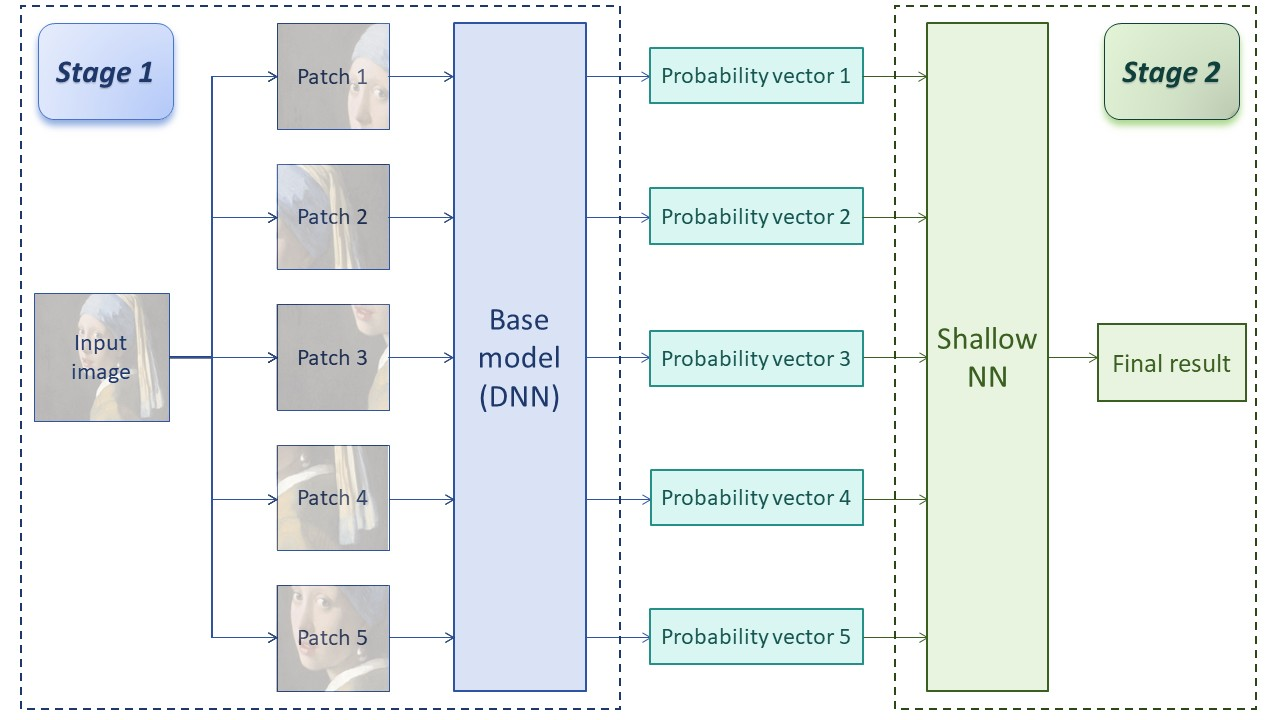
\includegraphics[width=0.5\textwidth]{fig/mainpipline.jpg}
    \caption{The architecture of the basic SNN adapter}
    \label{fig:architecture}
\end{figure}
The prediction consist of 2 stages. At the first stage, the image is dividing into 5 patches, as shown in Figure \ref{fig:patches}. The DNN independently 
classifies each of these five patches. In the second stage, the SNN functions as a decision-maker:  it takes the 
probability distributions generated by the DNN for the five patches as input and produces the final classification result.
\begin{figure}[h]
    \centering
    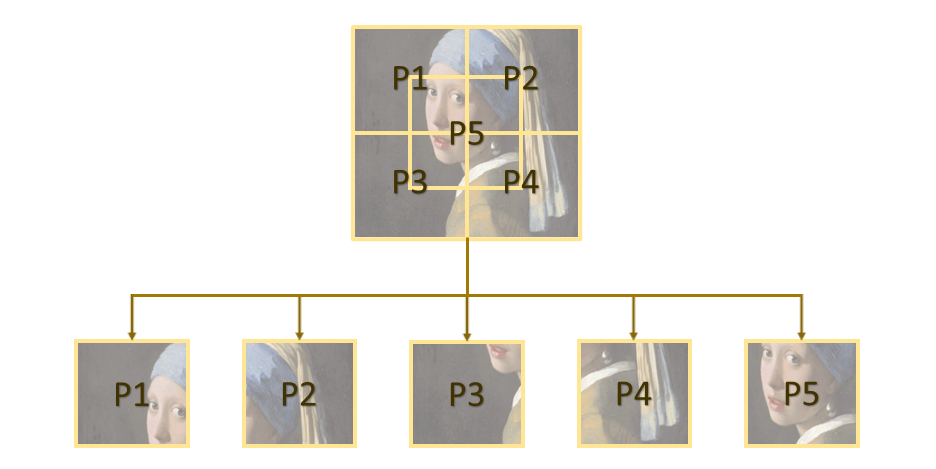
\includegraphics[width=0.5\textwidth]{fig/patch.png}
    \caption{Patch dividing of each image}
    \label{fig:patches}
\end{figure}

The proposed two-stage architecture combining a DNN and an SNN offers several key advantages:
\begin{itemize}
    \item It enables a more detailed examination of different regions within an artwork. By capturing fine-grained information and preserving important artistic details, this architecture enhances classification accuracy\cite{imran2023artistic}.
    \item Using probability vectors instead of images as inputs to the SNN reduces computational costs and avoids potential errors during image processing.
    \item The SNN functions as an independent decision-making adapter, making the model more flexible and generalizable. Since the DNN and SNN are trained independently, we can adjust their weights and architectures according to our needs. Each SNN adapter can fit different kinds of DNN models.
\end{itemize}

\subsection{Hierarchy SNN Architecture}
Despite the strong performance of the basic SNN adapter, it still faces certain limitations. Upon comparing the comprehensive prediction results of the DNN direct output and the SNN adapter output, we observed that while the SNN achieves higher overall accuracy, the DNN direct prediction exhibits superior accuracy in certain specific classes. 

To integrate the strengths of both networks, we proposed a two-layer hierarchical classification architecture. This architecture aims to extract both global and local features to generate the final prediction. The prediction pipeline is illustrated in Figure \ref{fig:hierarchical}.
\begin{figure}[h]
    \centering
    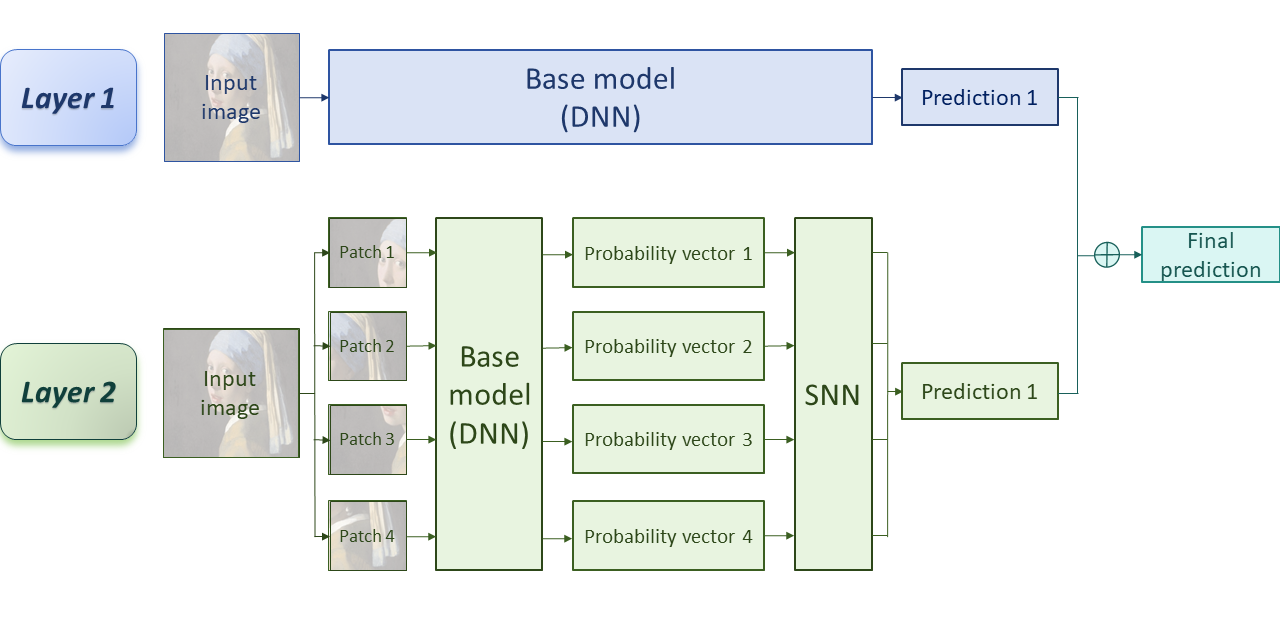
\includegraphics[width=0.5\textwidth]{fig/hierarchy.png}
    \caption{The architecture of the hierarchical SNN adapter}
    \label{fig:hierarchical}
\end{figure}

In this architecture, we employ a two-layer prediction scheme. In the first layer, the input image is fed directly into the base model (DNN), yielding the layer 1 prediction $p_{\text{layer1}}$ 
in the form of a probability vector. In the second layer, the input image is divided into four patches: left-top, left-bottom, right-top, and right-bottom. The DNN independently classifies each of these patches, generating probability vectors $p_1,p_2,p_3,p_4$. These probability vectors are then fed into the SNN adapter, which produces the layer 2 prediction 
$p_{\text{layer2}}$, also in the form of a probability vector.

The final prediction is a weighted sum of the predictions from the two layers:
\begin{align}
    p_{\text{final}} = w_1\cdot p_{\text{layer1}} + w_2\cdot p_{\text{layer2}},
\end{align}
where the weights $w_1$ and $w_2$ are proportional to the "reliability" of the respective layers. 
As suggested in \cite{hua2020artist}, the "reliability" can be evaluated based on the entropy of the probability vectors. Specificly, 
the entropy of the layer 1 prediction is calculated as:
\begin{align}
    H^1 &= -\sum_{i=1}^{C} p_{\text{layer1}}(i) \cdot \log(p_{\text{layer1}}(i)),
\end{align}
and the corresponding weight $w_1$ is given by:
\begin{align}
    w_1 &= 1 + 1/\exp(H^1),
\end{align}
For the second layer, the average probability vector $\overline{p}_{\text{layer2}}$ is fist computed as:
\begin{align}
    \overline{p}_{\text{layer2}}&=\frac{1}{4}(p_1 + p_2 + p_3 + p_4).
\end{align}
The entropy of the average probability vector is then calculated as:
\begin{align}
    H^2 &= -\sum_{i=1}^{C} \overline{p}_{\text{layer2}}(i) \cdot \log(\overline{p}_{\text{layer2}}(i)),
\end{align}
and the corresponding weight $w_2$ is given by:
\begin{align}
    w_2 &= 1 + 1/\exp(H^2).
\end{align}

\subsection{Patch Selection for SNN}
